\documentclass[fleqn,12pt]{article}
\usepackage[top=2cm, left=2cm,right=2cm,bottom=2cm]{geometry}%
\usepackage[fleqn]{amsmath}
\usepackage{amsmath,mathtools}
\usepackage{url,multicol}
%% ,enumerate}
%% \usepackage[shortlabels]{enumitem}
\usepackage{enumitem}
\setlist[enumerate]{leftmargin=12pt} 
\setlength{\mathindent}{0cm}
%\setlist[enumerate,0]{label=(\alph*),widest=a}
%[{\bf i.}]\begin{enumerate}[leftmargin=12pt]
\usepackage{ifthen}
\newboolean{answers}
%\setboolean{answers}{true}  % set to true to include TODO statements
\setboolean{answers}{false}  % set to false to use input statements
\usepackage{amssymb}
\usepackage{tikz}
\newcommand\rank{\ensuremath{\operatorname{rank}}}
\newcommand\nullity{\ensuremath{\operatorname{nullity}}}
\newcommand{\<}{\ensuremath{\langle}}
\renewcommand{\>}{\ensuremath{\rangle}}
\newcommand{\ur}{\ensuremath{\underline{\mathrm{r}}}}
\newcommand{\uT}{\ensuremath{\underline{\mathrm{T}}}}
\newcommand{\uF}{\ensuremath{\underline{\mathrm{F}}}}
\newcommand{\uN}{\ensuremath{\underline{\mathrm{N}}}}
\newcommand{\ui}{\ensuremath{\underline{\mathrm{i}}}}
\newcommand{\uj}{\ensuremath{\underline{\mathrm{j}}}}
\newcommand{\ua}{\ensuremath{\underline{\mathrm{a}}}}
\newcommand{\ub}{\ensuremath{\underline{\mathrm{b}}}}
\newcommand{\un}{\ensuremath{\underline{\mathrm{n}}}}
\newcommand{\uv}{\ensuremath{\underline{\mathrm{v}}}}
\newcommand{\R}{\ensuremath{\mathbb{R}}}
\newcommand{\ba}{\ensuremath{\mathbf{a}}}
%\newcommand{\bv}{\ensuremath{\mathbf{v}}}
\newcommand{\bb}{\ensuremath{\mathbf{b}}}
\newcommand{\bz}{\ensuremath{\mathbf{z}}}
\newcommand{\bw}{\ensuremath{\mathbf{w}}}
\newcommand{\bu}{\ensuremath{\mathbf{u}}}
\newcommand{\bv}{\ensuremath{\mathbf{v}}}
\newcommand{\bs}{\ensuremath{\mathbf{s}}}
\newcommand{\bx}{\ensuremath{\mathbf{x}}}
\newcommand{\bc}{\ensuremath{\mathbf{c}}}
\newcommand{\bi}{\ensuremath{\mathbf{i}}}
\newcommand{\bj}{\ensuremath{\mathbf{j}}}
\newcommand{\dotsize}{1pt}
\newcommand{\Heq}{\ensuremath{ \; \stackrel{\mathrm{H}}{=}} \; }
\begin{document}
\pagestyle{empty}



\noindent {\bf MATH 160} \hfill {\bf TEST 1} \hfill {\bf FALL 2015}
%% \hfill {\bf NAME:} \underline{\phantom{XXXXXXXXXXXXXXXXXX}}

%% ~ \hfill (print clearly)
\vskip1cm
\noindent {\bf RULES:}
\begin{itemize}
\item No books or notes or calculators allowed.
\item No bathroom breaks until after you have completed and turned in your test.
\item Out of consideration for your classmates, do not make
  disturbing noises during the exam. If you need a tissue, please ask for one.
\item {\bf Phones and other electronic devices must be off during the exam.}
\end{itemize}


\vskip2cm

\noindent    {\it Cheating will not be tolerated.}  If there is any indication that a
student may have given or received unauthorized aid on this test, the case 
will be handed over to the ISU Office of Judicial Affairs.
When you finish the exam, please sign the statement on the last page
acknowledging that you understand this policy.

\newpage

\begin{center}
  -scratch work-
\end{center}

\newpage

%\begin{enumerate}[label={\bf \arabic*.}]
\newgeometry{top=1cm, left=2cm,right=2cm,bottom=2cm}

\begin{flushright}
  Name: \underline{\phantom{XXXXXXXXXXXXXXXXX}}
\end{flushright}

\noindent {\bf Part 1.}
Complete the table by blacking out letters corresponding to correct answers.
%% \begin{multicols}{2}
  
  \begin{center}
    \begin{tabular}{|r|c|c|c|c|c|c|}
      \hline
      1. & (a) & (b) & (c) & (d) & (e) \\[4pt]
      \hline
      2. & (a) & (b) & (c) & (d) & (e) \\[4pt]
      \hline
      3. & (a) & (b) & (c) & (d) & (e) \\[4pt]
      \hline
      4. & (a) & (b) & (c) & (d) & (e) \\[4pt]
      \hline
      5. & (a) & (b) & (c) & (d) & (e) \\[4pt]
      \hline
    \end{tabular}
  \end{center}
%% \end{multicols}

\newcommand\probskip{\vskip2cm}

\bigskip

In Problems 1--4 assume $f(x) = (x-1)^3$.
(If the expression you are asked to compute is not defined or does not appear in
the list of possible answers, choose ``none of these.'')
\begin{enumerate}[label={\bf \arabic*.}]
\item Find the value of $f(x)$ when $x = -1$. 
  \\[6pt]
  (a) $-8$ \hfill (b) $-4$ \hfill (c) $0$ \hfill (d) $8$\hfill (e) none of these

  \probskip

\item What values of $x$ give a $f(x)$ value of $-1$.
  \\[6pt]
  (a) $-1$ \hfill (b) $0$ \hfill (c) $1$ \hfill (d) $2$\hfill (e) none of these

  \probskip

\item If $g(x) = \frac{1}{\sqrt{9-2x}}$, what is the value of $g(f(-1))$? 
  \\[6pt]
  (a) $-1/\sqrt{7}$ \hfill (b)  $1/\sqrt{17}$ \hfill (c)  $1/5$ \hfill (d)$1/3$ \hfill (e) none of these

  \probskip

\item
  Simplify the expression $\sqrt[3]{8r^6}\sqrt{s^4t^6}$. (Assume that $r$, $s$, and $t$ are positive.)\\[6pt]
  (a) $2r^2s^6t^4$\hfill (b) $8r^2s^2t^3$\hfill (c) $2r^2s^6t^3$ \hfill (d)$2r^2s^2t^3$
  \hfill (e) none of these %$8r^2s^4t^4$

  \probskip

\item Find the \emph{domain} of the function
  \[g(x) = \frac{\sqrt{x-6}}{x(x-8)}.\]
  %2x + 4}{x − 7}.
  (a) $[6, 8) \cup (8, \infty)$\hfill
    (b) $[6, \infty)$\hfill
      (c) $(8, \infty)$\hfill
      (d) $(-\infty, 0) \cup (0, 8) \cup (8, \infty)$\hfill
      (e) $(-\infty, \infty)$
      %% (-\infty, 7) \cup (7, \infty)
      %% (-\infty, -2) \cup (2, \infty)
      %% -\infty, - 2 \cup 2, \infty
      %% (-\infty, \infty)

%      \probskip

      %% \item 
      %% What is the \emph{domain} of the function $f(x) = \sqrt{6 - 9x}$?\\[6pt]
      %% (a) $(-\infty, \infty)$\hfill 
      %% (b) $(-\infty, 0]$\hfill 
      %% (c) $(-\infty, 1/3]$\hfill 
      %% (d) $(-\infty, 2/3]$\hfill 
      %% (e) none of these %$[0, \infty)$

      %% \probskip

\newpage
    \newgeometry{top=2cm, left=2cm,right=2cm,bottom=2cm}
\noindent {\bf Part 1.} (cont.)
Complete the table by blacking out letters matching correct answers.

  \begin{center}
    \begin{tabular}{|r|c|c|c|c|c|c|}
      \hline
      6. & (a) & (b) & (c) & (d) & (e) \\[4pt]
      \hline
      7. & (a) & (b) & (c) & (d) & (e)\\[4pt]
      \hline
      8. & (a) & (b) & (c) & (d) & (e)\\[4pt]
      \hline
      9. & (a) & (b) & (c) & (d) & (e) \\[4pt]
      \hline
      10. & (a) & (b) & (c) & (d) & (e) \\[4pt]
      \hline
      %%   11. & (a) & (b) & (c) & (d) & (e)  & (f)\\[4pt]
      %% \hline
      %%   12. & (a) & (b) & (c) & (d) & (e)  & (f)\\[4pt]
      %% \hline
    \end{tabular}
  \end{center}


    \item
      Find the \emph{range} of the function $f(x) = \sqrt{6 - 9x}$.\\[6pt]
      (a) $(-\infty, \infty)$\hfill
      (b) $(-\infty, 0]$\hfill
      (c) $[2/3,\infty)$\hfill
      (d) $(-\infty, 2/3]$\hfill
      (e) none of these %$[0, \infty)$ 

    \probskip

  \item Which function(s) has its domain identical with its range?
    (select all that apply)\\[6pt]
    (a) $f(x) = 1/x$
    \hfill (b) $g(x) = x$
    \hfill (c)  $h(x) = x^2$
    \hfill (d)  $i(x) = \sqrt{x}$
    \hfill (e) none of these

    \probskip

  \item Simplify the expression $|\sqrt{3} - 1| + |8 + \sqrt{3}|$.
    \\[6pt]
    (a) $7+2\sqrt{3}$\hfill 
    (b) $2\sqrt{3}$\hfill 
    (c) $9+2\sqrt{3}$\hfill 
    (d) $-2\sqrt{3}$\hfill 
    (e) none of these

    \probskip

    %% \item The equation of the line with slope 
    %% $m = -8$ and $y$-intercept $b = 3$ is
    %% \\[6pt]
    %% (a) $y = 8x -3$\hfill
    %% (b) $y = -8x +3$\hfill
    %% (c) $y = -8x -3$\hfill
    %% (d) $y = 3x - 8$\hfill
    %% (e) none of these

    %% \probskip

  \item The equation of the line that passes through the points
    $(2, 6)$ and $(3, 13)$ is
    \\[6pt]
    (a) $y = \frac{1}{7}x +\frac{8}{7}$\hfill
    (b) $y = -\frac{1}{7}x + \frac{20}{7}$\hfill
    (c) $y = -7x + 20$\hfill
    (d) $y = 7x - 8$\hfill
    (e) none of these

    \probskip

  \item Find the set of all $x$ values where the function $f(x)$  is continuous.
    \[
    f(x) = \frac{x^2-4}{x-2}
    \]
    (a) $(-\infty, \infty)$\hfill
    (b) $(-\infty, -2)$\hfill
    (c) $(2,\infty)$\hfill
    %(d) $x\neq 2$\hfill
    (d) $(-\infty, 2)\cup (2,\infty)$\hfill
    (e) none of these

    %\restoregeometry
%\begin{enumerate}[label={\bf \arabic*.}]
    \newpage

\newgeometry{top=1cm, left=2cm,right=2cm,bottom=2cm}

\begin{flushright}
  Name: \underline{\phantom{XXXXXXXXXXXXXXXXX}}
\end{flushright}

    \noindent {\bf Part 2.}
  \item In the following diagram, $S$ represents the position of a power relay
    station located on a straight coastal highway, and $M$ shows the location of a
    marine biology experimental station on an island. A cable is to be laid
    connecting the relay station with the experimental station. The cost of
    running the cable on land is \$3/running foot and the cost of running cable
    under water is \$5/running foot.  

    \begin{center}
      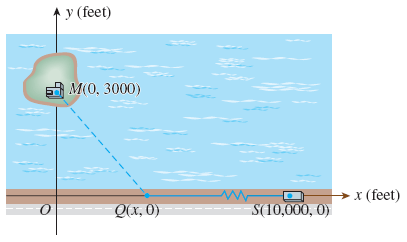
\includegraphics[height=3in]{1-3-040}
    \end{center}

    \begin{enumerate}[label={\bf \roman*.}]
    \item (4pts) Find an expression in terms of $x$ that gives the total cost of 
      laying the  cable.  

      \vskip4cm
      
      \hfill {\bf Answer:} 
      $C(x) = $\phantom{XXXXXXXXXXXXXXXXXXXXXXXX}\\
      \phantom{X}  \hfill \underline{\phantom{XXXXXXXXXXXXXXXXXXXXXXX}}
      % Ans: C(x) =  3(10000 - x) + 5(sqrt(x^2 + 3000^2))

      \bigskip

    \item (3pts) What is the total cost when $x = $ 4,000? 

      \vfill

      \hfill {\bf Answer:} 
      $C(4000) = $\phantom{XXXXXXXXXXXXXXXXXX}\\
      \phantom{X}  \hfill \underline{\phantom{XXXXXXXXXXXXXXXX}}
      % Ans: C(4000) =  3(10000 - 4000) + 5(sqrt(16000000 +9000000))
      %           =  3(6000) + 5(sqrt(25000000))
      %           =  18000 + 5(5000))
      %           =  18000 + 25000
      %           =  43000
    \end{enumerate}

    %% \newpage

    %% \item All parts of this question concern the function $f(x) = \frac{1}{x}$

    %% \begin{enumerate}[label={\bf \roman*.}]
    %% \item Compute the limit of $f(x) = 1/x$ as $x$ approaches infinity, as $x$
    %%   approaches zero from the right, and as $x$ approaches
    %%   negative infinity.  (You don't need to show your work for this part.)

    %% \hfill {\bf Answers:} 
    %% $\lim\limits_{x\rightarrow \infty} f(x) = $\phantom{XXXXXXXXXXXXXX}\\
    %% \phantom{X}  \hfill \underline{\phantom{XXXXXXXXXXXXXX}}

    %% \vskip5mm

    %% \hfill \phantom{{\bf Answers:} } 
    %% $\lim\limits_{x\rightarrow 0^+} f(x) = $\phantom{XXXXXXXXXXXXXX}\\
    %% \phantom{X}  \hfill \underline{\phantom{XXXXXXXXXXXXXX}}

    %% \vskip5mm

    %% \hfill \phantom{{\bf Answers:} } 
    %% $\lim\limits_{x\rightarrow -\infty} f(x) = $\phantom{XXXXXXXXXXXXXX}\\
    %% \phantom{X}  \hfill \underline{\phantom{XXXXXXXXXXXXXX}}

    %% \bigskip

    %% \item
    %% Find the equation of the line tangent to the graph of $f(x) = 1/x$ at the point 
    %% $(x, f(x)) = \left(\frac{1}{2},2\right)$.
    %% Present your answer in $y = mx + b$ form.
    %% \\\\
    %% {\it Your work:}

    %% \vskip6cm


    %% \hfill {\bf Answer:} $y = $ \phantom{XXXXXXXXXXXXXX}\\
    %% \phantom{X}  \hfill \underline{\phantom{XXXXXXXXXXXXXX}}
    %% \end{enumerate}

    \newpage
    \newgeometry{top=2cm, left=2cm,right=2cm,bottom=2cm}


    % Problem 2.3.24 and 2.6.21
  \item (15pts) Evaluate each limit. If the limit does not exist, write
    DNE. (Show your work!)
    \begin{enumerate}[label={\bf \roman*.}]


    \item 
      \label{item:2}
      \[
      \lim_{x\rightarrow 2} \frac{2x^2 + 1}{x^2 +5x - 4}
      \]
      %% answer: 9/10

      \bigskip

      \bigskip
      \hfill {\bf Answer:} \underline{\phantom{XXXXXXX}}
      \bigskip

      %--------------------

    \item 
      \label{item:3}
      \[
      \lim_{x\rightarrow -1} \frac{x^2 - 4x}{x^2 -3x - 4}
      \]
      %% answer: DNE

      \bigskip

      \bigskip
      \hfill {\bf Answer:} \underline{\phantom{XXXXXXX}}
      \bigskip

      %--------------------

      \bigskip
    \item 
      \label{item:4}
      \[
      \lim_{x\rightarrow -2} \frac{x^2 + 4x + 4}{x^4 -16}
      \]

      \bigskip

      \bigskip
      \hfill {\bf Answer:} \underline{\phantom{XXXXXXX}}
      \bigskip

      %--------------------

      \bigskip
    \item 
      \label{item:5}
      \[
      %\lim_{x\rightarrow \infty} \frac{8x^4 + 3}{(x^2-2)(7x^2 -1)} 
      \lim_{y\rightarrow \infty} \frac{1-3y^2}{2y^2+5y} 
      \]
      % answer: -3/2

      \bigskip

      \bigskip
      \hfill {\bf Answer:} \underline{\phantom{XXXXXXX}}
      \bigskip

      %--------------------

      \bigskip
    \item 
      \label{item:6}
      \[
      \lim_{x\rightarrow \infty} (x - \sqrt{x^2 + 6x})
      \]

      \bigskip

      \bigskip
      \hfill {\bf Answer:} \underline{\phantom{XXXXXXX}}
      \bigskip

      %--------------------


    \end{enumerate}

    \newpage
%\begin{enumerate}[label={\bf \arabic*.}]
\newgeometry{top=1cm, left=2cm,right=2cm,bottom=2cm}

\begin{flushright}
  Name: \underline{\phantom{XXXXXXXXXXXXXXXXX}}
\end{flushright}

  \item (4pts) For what value of $k$ will the function $f$ be continuous on 
    $(-\infty,\infty)$? (You must justify your answer and show your work in order to
    receive credit on this problem.)
    \[
    f(x) = 
    \begin{cases}
      \frac{x^2 - 16}{x + 4}, & \text{ if } x \neq -4,\\
      k, & \text{ if } x = -4.
    \end{cases}
    \]

    \vskip4cm

    \hfill {\bf Answer:} $k = $ \underline{\phantom{XXXXXXXXXX}}

    \vskip1cm

  \item (4pts) Consider the graph of a function shown below.  
    Identify the domain of the function and the set of values at which the
    function is continuous. (Circle letters next to correct answers.)
    %% Indicate the interval(s) on which this function is continuous by writing a
    %% checkmark next to each such interval. 

    \begin{center}
      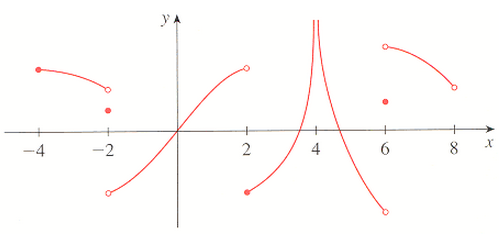
\includegraphics[height=3in]{Problem254}
    \end{center}
    
    \begin{multicols}{2}

      The {\bf domain} of the function:
    \begin{enumerate}[label=(\alph*)]
    \item $[-4, 8)$
    \item $[-4, 4)\cup(4,8)$
    \item $(-\infty, -4) \cup [8,\infty)$
    \item $[-4, -2)\cup(-2,2) \cup [2,6) \cup (6,8)$
      \item $[-4, -2)\cup(-2,2) \cup (2,4) \cup (4,6)\cup (6,8)$
    \end{enumerate}

    $x$ values where the function is {\bf continuous}:
    \begin{enumerate}[label=(\alph*)]
    \item $[-4, 8)$
    \item $[-4, 4)\cup(4,8)$
    \item $(-\infty, -4) \cup [8,\infty)$
    \item $[-4, -2)\cup(-2,2) \cup [2,6) \cup (6,8)$
      \item $[-4, -2)\cup(-2,2) \cup (2,4) \cup (4,6)\cup (6,8)$
    \end{enumerate}

    \end{multicols}
\end{enumerate}

\newpage

\noindent {\bf MATH 160} \hfill {\bf TEST 1} \hfill {\bf FALL 2015}

\vskip1cm

\noindent    {\it Cheating will not be tolerated.}  If there is any indication
that a student may have given or received unauthorized aid on this test, the
case will be handed over to the ISU Office of Judicial Affairs. When you finish
the exam, please sign the following statement acknowledging that you understand
this policy:\\
\\
``On my honor as a student I,
\underline{\phantom{XXXXXXXXXXXXXXXXXXXXXX}}, have neither
given nor received unauthorized aid on this exam.''
\hbox{} \hskip .25cm {\small (print name clearly)}\\
\\
\begin{flushright} Signature: \underline{\phantom{XXXXXXXXXXXXXXXXXXXXXXXXXXXXXX}}
  Date: \underline{\phantom{x} 2015-09-22 \phantom{x}}
\end{flushright}


\vfill

\hrule

\begin{center}
(do not write below this line)  
\end{center}


\vskip1cm

\begin{flushright}
% \begin{center}
  {\Large
    \begin{tabular}{r|r|r|l}
probs&      page   & max  & score\\[4pt]
      \hline
      1--5.&  1&15&\\[4pt]
      \hline
      6--10.&  2&15&\\[4pt]
      \hline
      11. & 3&7&\\[4pt]
      \hline
      12. &4& 15&\\[4pt]
      \hline
      13, 14. & 5 &8&\\[4pt]
      \hline
     & Total  &60&
    \end{tabular}
  }
\end{flushright}
%% \end{center}

\vskip2cm


\end{document}

